
\textbf{\textit{The Models}}---
%Nevertheless the study can also be applied to sterile neutrinos via magnetic portal, as we discuss in the Supplementary Materials. For the case of sterile neutrino with mixing portal, special care needs to be taken for resonant conversions in which case active neutrinos with plasma mass would travel as slowly as the sterile neutrinos at specific distances.
Let us consider the Majoron model, studied in \cite{Fiorillo:2022cdq}, where supernova 1987A constraints were derived. The relevant part of the Lagrangian reads
\begin{align}
\mathcal{L} \supset -\frac{g_{\alpha\beta}}{2} \nu_\alpha \nu_\beta \phi - m_\phi \phi\phi^* + \text{h.c.}\,,
\end{align}
where $\phi$ is the (pseudo)scalar, $m_\phi$ is the respective mass and $g$ parametrizes interaction strength between $\phi$ and neutrinos. We assume flavor universal interaction and hence $g_{\alpha\beta}\equiv g_\phi \, \delta_{\alpha\beta}$. Majorons are produced from (anti)neutrino coalescence in the star and subsequently decay to a pair of (anti)neutrinos resulting in BSM (anti)neutrino flux emitted from the star. The total decay width is given by $\Gamma_\phi = 3g^2 m_\phi/16 \pi$.

We will set SN bounce time $t_{\rm bounce}$ as $t = 0$. Using data from the simulation of $8.8 M_\odot$ progenitor star \cite{Huedepohl2010, Garching} and including effects of neutrino oscillations assuming normal mass ordering, we calculated standard neutrino fluxes at Earth that can be presented in terms of the parametrization with the ``pinching'' factor \cite{Keil:2002in,baxter2021snewpy}. Following \cite{Fiorillo:2022cdq}, we also calculated the flux of emitted Majorons. At $t \leq \unit[0.05]{s}$, Majorons are mainly produced through 
$\nu_e$ and $\nu_x$ coalescence with $\nu_x$ including (anti)neutrinos of $\tau$ and $\mu$ flavor. 
After $\unit[0.05]{s}$, the flux of Majorons decreases as the total flux of neutrinos of all flavors. Thus we found that Majoron flux peaks around $t \sim \unit[0.05]{s}$.
We further cross checked the agreement with \cite{Fiorillo:2022cdq} by reproducing the bound from SN energy loss criteria. 

Very weakly coupled Majorons immediately stream out after the production. On their way to Earth, Majorons of energy $E_\phi$ will travel at the speed of $\beta$ for a distance of $L_1$, then decay to (anti)neutrinos of energy $E_\nu$ at an emission angle $\cos\alpha = (2 E_\phi E_{\nu} - M^2_N)/(2E_{\nu}E_\phi\beta)$. Daughter (anti)neutrino will travel for a distance $L_2$ and reach the Earth at the angle $\theta$ satisfying $D_{\rm SN} \sin\theta = L_1 \sin\alpha$ for a SN that is $D_{\rm SN}$ away (see such geometry in \cite{Brdar:2023tmi}). The time delay, $\delta t$, relative to a relativistic particle moving along the line-of-sight path from SN to reach the Earth is given by
\cite{Jaeckel:2017tud}
\begin{align}
    \delta t = (\frac{L_1}{\beta}-L_1) + (L_1 + L_2 -D_{\rm SN})\,,
    \label{eq:deltatexa}
\end{align}
where we have split the contribution to $\delta t$ into two parts: the first part comes from the slowly moving of Majorons before its decay, and the second part is due to the detour from the line-of-sight path at the given emission angle $\alpha$. 

To get the characteristic value of $\delta t$, we can take $L_1 = L_\phi$ with $L_\phi = (E_\phi/m_\phi) \Gamma^{-1}_\phi \beta$ being the decay length of $\phi$. As for the parameter regions we considered, $(D_{\rm SN} -D_{\rm SN} \cos\theta) \ll \unit[10^{-3}]{s}$, $\delta t$ can be approximated
\begin{align}
    \delta t &\simeq L_\phi(\frac{1}{\beta} -1) + L_\phi(1-\cos\alpha) = \frac{8\pi}{3 E_{\bar{\nu}_{e}}g_\phi^2}\,,
    \label{eq:deltat}
\end{align}
which is roughly independent of Majoron energy $E_\phi$. However, at small values of $E_\phi$, the main contribution to $\delta t$ comes from the first term due to slowing moving Majorons, while at larger values of $E_\phi$, from the second term due to larger detour given the increase of $L_\phi$ over the decrease of $(1-\cos\alpha)$.
%For neutrinos from light Majoron decay, the characeristic time delay is set by the detour, while for   
%We have $L_1 \lesssim L_\phi$ with $L_\phi = (E_\phi/m_\phi) \Gamma^{-1}_\phi \beta$ being the decay length of $\phi$.
%As $L_\phi$ is much smaller than $D_{\rm SN}$ for all values of $E_\phi$ and the parameter regions considered, we can estimate that $(D_{\rm SN} -D_{\rm SN} \cos\theta) \ll \unit[10^{-3}]{s}$. Thus we can approximate $\Delta t$ as
%\begin{align}
%    \delta t &\simeq L_1/\beta -L_1 \cos\alpha\ \\\notag
%    &= (L_1/\beta -L_1) + (L_1-L_1 \cos\alpha)\,.
%    \label{eq:deltat}
%\end{align}
%Taking $L_1 \simeq L_\phi$, we have $\Delta t \sim 8\pi/(3 E_e g_\phi^2)$. 

We can obtain the flux of daughter $\nu$ by considering decays that occur only at $R^{\nu}_{\rm SN}\leq L_1$. As the smallest decay distance beyond which the daughter neutrino can escape the explosion unperturbed, we take $R^{\nu}_{\rm SN} = \unit[30]{km}$. We will also limit our analysis to a maximal time window of $\unit[100]{s}$ after SN bounce. This time window is larger than typical values of time delay considered for the parameter space in consideration.
\begin{figure}[t!]
    \centering
    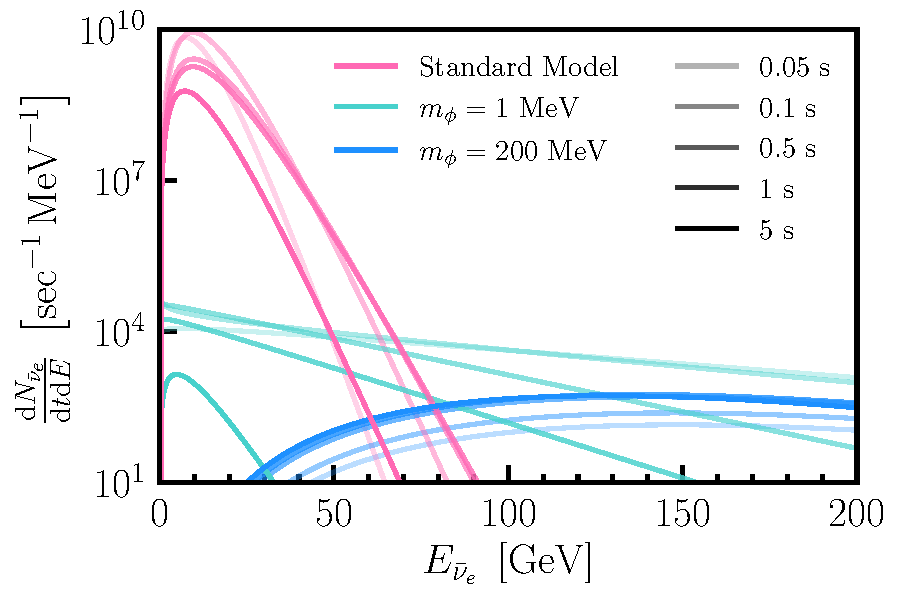
\includegraphics[width=0.47\textwidth]{figures/majoran_fluxes.pdf}
    \caption{\textit{\textbf{Flux of $\bar{\nu}_{e}$ from Standard Model production and two majoron hypotheses}}.
    We choose the parameters $g_\phi = 10^{-10.2}$ and $g_\phi = 10^{-11.8}$ for $m_\phi = \unit[1]{MeV}$ and $m_\phi = \unit[200]{MeV}$, respectively. \yy{the unit for the x-axis should be MeV, for y-axis, we chose to use $\rm s$ for second instead of $\rm sec$.}
    }
    \label{fig:fluxes}
\end{figure}
We will consider a SN event that happens in the galaxy at a distance $D_{\rm SN}=\unit[10]{kpc}$, which is not unlikely~\cite{Reed:2005en,Rozwadowska:2020nab}. As $\bar{\nu}_e$ contribute chiefly to the signals at IceCube via inverse beta decay (IBD), we show in \cref{fig:fluxes} the differential fluxes of daughter $\bar{\nu}_e$ at different time for two benchmark points in the Majoron model, in comparison to the SM $\bar{\nu}_e$ flux. We expect the observed signal timing distribution at IceCube to follow these patterns of $\bar{\nu}_{e}$ flux. 

From \cref{fig:fluxes}, we can observe that the energy of $\bar{\nu}_e$ from Majoron decay extends to $\unit[100]{MeV}$ and above for both benchmarks, as expected. 
Consider the light Majoron case in \cref{fig:fluxes}. Majorons, generating neutrinos with $E_{\bar{\nu}_e} \geq \unit[150]{MeV}$, are nearly-relativistic with the emission angle $\alpha$ close to zero. The time delay can be estimated from the first term in \cref{eq:deltat} given by $\delta t \sim L_\phi (1/\beta -1)\lesssim \unit[0.01]{s}$. With such a negligible time delay, the time dependence of the $\bar{\nu}_e$ flux is mainly inherited from that of the Majorons upon production, with larger fluxes at $t\leq \unit[0.05]{s}$. Notice that such $\bar{\nu}_e$ flux would arrive at the detector earlier than the peak of the SM $\bar{\nu}_e$ flux which is around $t\simeq \unit[0.1]{s}$ from \cref{fig:fluxes}, it potentially leads to early signals at IceCube.
%For $\bar{\nu}_e$ produced with energy, i.e $E_{\bar{\nu}_{e}} \sim \unit[10]{MeV}$, a fraction of their mother Majorons will have energy $E_\phi\sim\mathcal{O}(\unit[10]{MeV})$, resulting in typical $\delta t \gtrsim \unit[0.1]{s}$. For higher values of $E_\phi$, the main contribution from detour also leads to $\delta t \gtrsim \unit[0.1]{s}$. 
The time delay for $\bar{\nu}_e$ with energy, i.e $E_{\bar{\nu}_{e}} \sim \unit[10]{MeV}$ is typically $\gtrsim \unit[0.1]{s}$ from \cref{eq:deltat}. These $\bar{\nu}_e$ could be produced from Majorons with low energy of $\mathcal{O}(\unit[10]{MeV})$ or high energies. For the low energy Majoron case, the time delay is mainly due to slowly moving Majoron, while for high energy case, mainly from the detour.
Such sizable time delay will shift $\bar{\nu}_e$ peak flux to later time, in comparison to that of their mother Majorons, as exhibited in \cref{fig:fluxes}.

For heavy Majoron case, the resulting $\bar{\nu}_e$ flux is larger at later time, manifesting the time delay from slowly moving Majorons. For the heavy Majoron benchmark in \cref{fig:fluxes}, we can estimate that $\delta t \gtrsim \unit[10]{s}$ for $E_{\bar{\nu}_{e}}\sim \unit[200]{MeV}$ which is delayed comparing to the peak of SM $\bar{\nu}_e$ flux. Comparing to the light Majoron case, such large time delay is a combination of a more slowly moving Majoron and a larger detour due to its large emission angle. As $L_1\lesssim L_\phi$, the time spread of the flux is roughly given by the aforementioned characteristic value of time delay which is $\unit[0.1]{s}$ ($\gtrsim\unit[10]{s}$) for the light (heavy) benchmark case.
%which yield sizable $\bar{\nu}_e$ flux extending to sizeable $t$.
%in details in the following, we consider energy deposits at the photomultipliers, 
%due to denser and hotter core of SN  as Majorans shortly after the bouncing time $t_{\rm bounce}$ from the hot dense core of SN. 

% \begin{figure*}
%     \centering
%     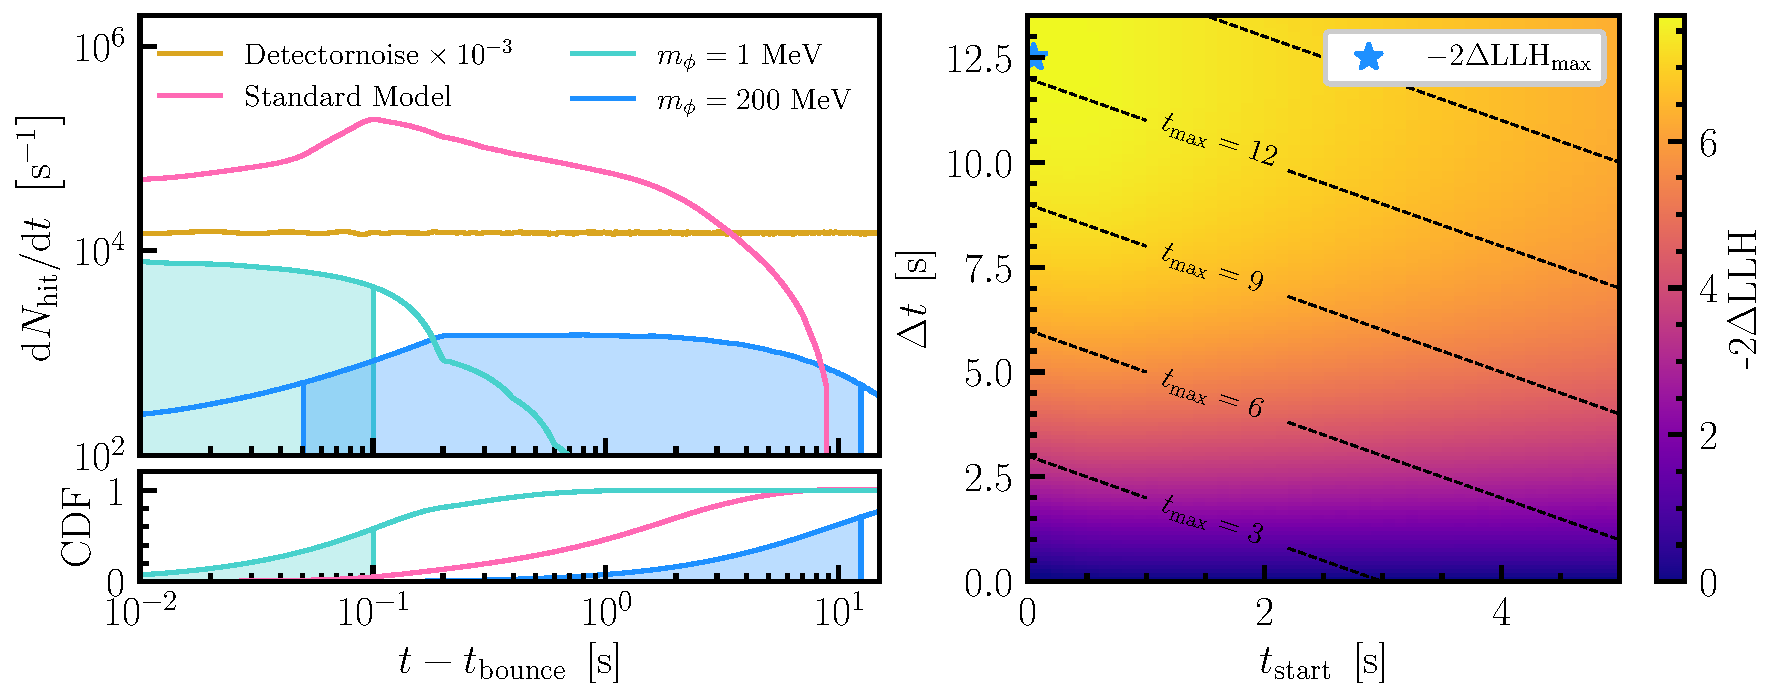
\includegraphics[width=0.95\textwidth]{figures/hits_and_likelihood.pdf}
%     \caption{\textbf{\textit{Timing profile of hits and test statistic as a function of the timing window.}}
%     These are the same points in the parameter space as Fig.~\ref{fig:fluxes}.
%     }
%     \label{fig:hits_and_likelihood}
% \end{figure*}
